%% Group 3: KVCache-Coordinated Latency Optimization for LLM Inference Serving
%% CSCI 6806 Graduate Capstone -- Final Report
%%
%% Build:  make    (or: pdflatex main && bibtex main && pdflatex main && pdflatex main)

\documentclass[conference]{IEEEtran}
\IEEEoverridecommandlockouts

\usepackage[T1]{fontenc}
\usepackage{cite}
\usepackage{graphicx}
\usepackage{booktabs}
\usepackage{amsmath}
\usepackage{url}
\usepackage[table]{xcolor}
\usepackage{float}

\graphicspath{{figures/}}

\renewcommand{\topfraction}{0.95}
\renewcommand{\bottomfraction}{0.95}
\renewcommand{\textfraction}{0.05}
\renewcommand{\floatpagefraction}{0.80}
\renewcommand{\dbltopfraction}{0.95}
\renewcommand{\dblfloatpagefraction}{0.80}
\setcounter{topnumber}{3}
\setcounter{dbltopnumber}{3}
\setcounter{totalnumber}{5}

\setlength{\textfloatsep}{6pt plus 2pt minus 2pt}
\setlength{\floatsep}{6pt plus 2pt minus 2pt}
\setlength{\intextsep}{6pt plus 2pt minus 2pt}
\setlength{\abovecaptionskip}{4pt}
\setlength{\belowcaptionskip}{0pt}

\begin{document}

\title{Group 3: KVCache-Coordinated Latency\\ Optimization for LLM Inference Serving}

\author{%
\IEEEauthorblockN{Guoliang Liu, Wenhui Kang, and Junpeng Huang}
\IEEEauthorblockA{Fairleigh Dickinson University \textit{Vancouver Campus, Canada}}
}

\maketitle

\begin{abstract}
Large language model serving has an important memory problem. During generation, every new token needs to read all previous key-value cache blocks. As context length and concurrent requests increase, GPU memory becomes full before the GPU computation is fully used. When the cache pool is full, the serving engine must preempt requests. It can either swap the cache to memory or delete the cache and recompute it later. Both choices increase latency, especially under high request load. Learning-to-rank scheduling improves request ordering, but it does not reduce the memory cost of each request.

This project combines a learning-to-rank scheduler with two KV-cache optimizations: TurboQuant's 4-bit KV cache quantization and BLASST's attention sparsity in the decode kernel. Quantization increases the number of cache tokens that fit in the same GPU memory, while sparsity skips attention blocks with non-important small softmax contribution. At 64 requests per second, our combined cache design reduced mean time-to-first-token from 12,275 ms to 1,747 ms and reduced preemptions from 162 to 40 per run. The sparsity optimization also reduced mean per-token latency by 22.1\% and P99 per-token latency by 46.8\% on the per-head decode kernel. However, the same sparsity method was harmful on a grouped-query kernel, which shows that the kernel implementation strongly affects the final benefit.
\end{abstract}

\clearpage
\section{Introduction}

Large language models (LLM) are used for chat systems, coding assistants, document analysis, and many other applications now. However, serving an LLM efficiently is difficult. During autoregressive generation, the model produces one token at a time, and for every new token it attends to all previous tokens. To avoid recomputing the previous key and value (KV) projections, serving engines store them in a KV cache. This cache grows with context length and with the requests rate. Therefore, GPU memory (VRAM) often becomes the main bottleneck before GPU computation does.

PagedAttention improved LLM serving by dividing KV cache memory into fixed-size blocks and allocating blocks when needed~\cite{vllm2023}. This design reduces memory fragmentation and allows more requests throughput. However, the cache pool is limited. When the pool becomes full, the serving engine must preempt one or more requests. Some engine versions swap cache blocks to host memory. Other versions remove the cache and later recompute the request prefill. Both methods are expensive. While swapping is limited by the host--device bandwidth, recomputation repeats the prompt processing work. Overall, these costs appear under high load, where low latency matters most.

Request scheduling is one solution. Learning-to-rank (LTR) scheduling predicts which requests will likely generate shorter outputs and gives them higher processing priority. This reduces head-of-line (HOF) blocking, because short requests do not wait behind long requests, also known as shortest-job-first (SJF). Previous work reported up to around 2.1 times latency reduction compared with first-come-first-serve (FCFS) scheduling at high load~\cite{fu2024ltr,kumar2026}. However, scheduling does not change how much GPU memory each request needs. It only changes which request runs first. When memory is already full, ordering algorithms cannot eliminate the memory pressure.

KV cache quantization is another solution. It reduces the number of bytes needed for each cache token. TurboQuant uses rotation-based low-bit quantization to make low-bit KV cache memory-efficient~\cite{turboquant2025}. KVmix uses different bit widths for layers with different sensitivity~\cite{kvmix2026}. These approaches improve capacity, but quantization adds unpacking and dequantization computation work during decoding. Therefore, cache compression methods can improve time-to-first-token (TTFT) while making per-token latency (TPOT) worse.

Attention sparsity can reduce decode computation. BLASST uses the running maximum already maintained by streaming softmax and skips attention blocks whose scores are too small to meaningfully affect the output~\cite{blasst2025}. This method is useful because it does not need a separate predictor or an extra attention pass. However, algorithmic sparsity is not always equal to real kernel speedup. A kernel can skip a block only when its tile structure allows the block to be skipped for all grouped operations.

Our project studies these methods as one serving system instead of evaluating each method separately. We place a KV cache layer below an LTR scheduler. The cache layer includes 4-bit KV cache quantization and a softmax-threshold attention sparsity method. We measure average latency, TTFT, TPOT, tail latency, cache occupancy, and preemption count. The detailed works are as follows:

\begin{itemize}
  \item We built a KV cache optimization layer under a learning-to-rank scheduler using supported serving-engine interfaces.
  \item We reproduce the LTR scheduling result on the original engine and workload configuration.
  \item We evaluate cache compression across three vLLM versions with swap and recomputation preemption strategies.
  \item We show that cache compression reduces memory pressure and preemptions, while attention sparsity can recover part of the decode cost caused by low-bit cache storage.
  \item We show that attention sparsity depends on kernel tiling: it improves the per-head kernel but hurts the grouped-query attention (GQA) kernel.
  \item We explain that swapping and cache compression are two different ways to handle the same KV cache memory pressure.
\end{itemize}

\clearpage
\section{Background}

\subsection{Paged Key--Value Cache and Preemption}

A decoder-only transformer generates output one token at a time. When it generates token t, the model attend to the keys and values of tokens 1 through t $-$ 1. Recomputing these values at every step is very expensive. Therefore, serving engines store the previous keys and values in a KV cache.

PagedAttention stores KV cache data in fixed-size blocks instead of allocating one large continuous memory block for each request~\cite{vllm2023}. This matters because the output length is unknown when a request begins. A continuous allocation would either reserve too much memory or need memory copying later. With paged allocation, each request receives more blocks only when it needs them, and the wasted memory is limited to at most one partially used block per request.

Figure~\ref{fig:arch-preempt} shows the basic serving path. Requests first enter the scheduler. The scheduler selects the next request, and the block allocator gives KV cache blocks to that request. During decoding, the attention kernel repeatedly reads previous KV blocks. If the cache pool is full, the serving engine preempts a request. One option is swapping, where cache blocks move from GPU memory to host memory. Another option is recomputation, where the engine deletes the cache and reruns prefill when the request resumes.

\begin{figure}[H]
  \centering
  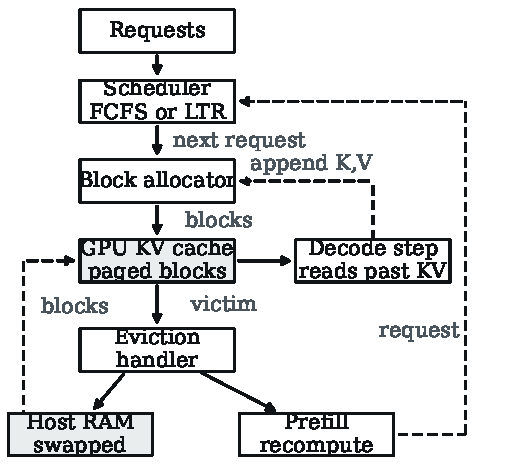
\includegraphics[width=\columnwidth]{arch_preempt.pdf}
  \caption{Serving data path and the two preemption routes. Requests are ordered by the scheduler, the block allocator draws fixed-size blocks from the paged key--value pool, and the attention kernel reads them on every decode step. When the pool is exhausted a victim is either swapped to host memory and copied back or evicted and recomputed from its prompt.}
  \label{fig:arch-preempt}
\end{figure}

The two recovery paths act differently under load, and this difference matters later in the paper. Firstly, while swapping moves cache blocks over the host--device link, its cost grows with the size of the cache, but the link bandwidth is limited. Moreover, while recomputation reruns the prefill, its cost grows with the length of the prompt. Thus, recomputation punishes long requests the most, and length-aware scheduler tends to delay long requests. Older vLLM engine offered both paths, but we use vLLM 0.25 for our main experiments keeps only recomputation. Later, we show that this choice changes how well the earlier scheduling result behaves in a newer engine. The cache pool is also limited, and its occupancy is the product of two things: how many requests run at the same time, and how long each request has become. As a result, admission is controlled by memory rather than by computing.

When the allocator cannot find free blocks for a new request, the engine must preempt an existing one. Therefore, the memory pressure decides how many requests a single device can serve at once, which is the factor both of our cache features try to reduce.

\subsection{KV Cache Quantization}

KV cache data uses a large amount of memory because it stores activations for every generated token. Low-bit quantization reduces the memory used by the cache. However, KV activation can contain outliers. If one large value controls the quantization scale, many low-bit levels are wasted on the smaller values.

Rotation-based quantization helps solve this issue. An orthogonal rotation spreads the outlier energy across dimensions while preserving inner products in exact arithmetic. TurboQuant applies this idea to online vector quantization and achieves low distortion at low bit widths~\cite{turboquant2025}. KVmix improves the idea by using more bits for sensitive layers and fewer bits for less sensitive layers~\cite{kvmix2026}. There is also an asymmetry between keys and values. Specifically, while errors in keys are amplified by the exponential in the softmax, errors in values enter the output only linearly. Thus, keys and values do not need to be stored at the same precision.

The main benefit of 4-bit cache storage is capacity. With the same memory budget, in our configuration the 4-bit cache holds 2.83 times more tokens than the bfloat16 (BF16) cache. However, the cost is that every decode step must read, unpack, and dequantize the low-bit cache data. Therefore, cache quantization reduces queueing latency but increases per-token decode latency.

\subsection{Streaming-Softmax Attention}

Attention computes a score between a query and each previous key. These scores are normalized by softmax, and combined using the normalized weights afterwards. A normal softmax implementation must store all scores before computing the final result, which requires large temporary memory for long contexts.

Streaming softmax solves this problem by processing attention one block at a time. The kernel keeps three running values: the current maximum score, the softmax denominator, and the weighted value accumulator. When a new key block has a larger maximum score, the previously accumulated values are rescaled. This process gives the same mathematical result while using constant temporary memory.

During rescaling, the kernel keeps three numbers as it reads the key blocks: the largest score seen so far, the running softmax denominator, and the running weighted sum of values. When a new block produces a larger maximum, the kernel multiplies the denominator and the value sum by the exponential difference between the old and new maximum. This moves everything already added to the new reference point. The correction costs one multiplication per block, which is small compared to the matrix products it protects, and the final result is exact rather than estimation.

\begin{figure}[H]
  \centering
  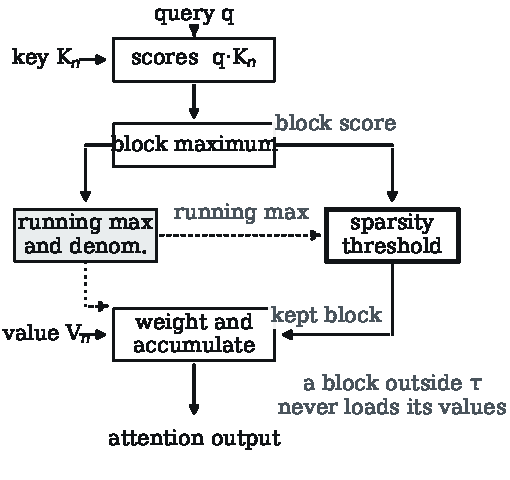
\includegraphics[width=\columnwidth]{arch_attention.pdf}
  \caption{Streaming-softmax attention and the sparsity gate. Blocks of KVs arrive at the kernel, which maintains a running maximum and denominator and rescales its accumulator as each block is folded in. The threshold test compares a block's own maximum against the running maximum and gates the value load and the second matrix product; the query--key product cannot be skipped because it produces the quantity being tested.}
  \label{fig:arch-attention}
\end{figure}

Eventually, the running maximum is used for sparsity. If the best score in a KV block is much lower than the running maximum, the block has almost no softmax contribution, so the kernel skip the value loading and accumulation for this block. However, it cannot skip the query--key computation, because the score must be computed before the kernel knows whether the block is important. Skipping a block avoids the softmax arithmetic, the value load, and the second matrix product, but it does not avoid the query--key product that created the score being tested. Thus, this limits the largest possible saving to about half of the attention work, which is why the benefit of sparsity depends on whether decoding is arithmetic-bound or bandwidth-bound. Figure~\ref{fig:arch-attention} shows this structure and the point where our sparsity method attaches.

\subsection{Learning-to-Rank Scheduling}

SJF scheduling can minimize the average waiting time, but an LLM server does not know the final output length before generation finishes. LTR scheduling solves this problem by predicting the relative output length of requests instead of the exact length~\cite{fu2024ltr}. The scheduler only needs to know which request is likely shorter. Predicting an order is easier than predicting a length. The ranker is trained with a listwise objective that scores a whole list of requests at once and penalizes any ordering that disagrees with the observed output lengths. Its quality is reported as a rank correlation rather than length-prediction error, because only the order matters for scheduling.

In this project, an OPT-125M ranking model gives each prompt a priority score. The score is mapped to a request priority and consumed by engine's existing priority policy. Since no engine internals have changed, the scheduling policy is replaced without modifying the block allocator that the cache levers act on. Since shorter requests can finish earlier, HOF blocking is reduced. Also, cache exhaustion is delayed, because fewer long requests are active at the same time.

However, LTR scheduling has a limitation since long requests are delayed by design. On an engine that uses recomputation, a delayed request can be preempted and forced to redo its refill later. This cost mainly affects high percentile latency. Therefore, we evaluate both mean and tail latency.

\clearpage
\section{Related Work}

\subsection{KV Cache Compression}

TurboQuant uses a rotation-based quantization method to reduce KV cache storage while keeping low distortion~\cite{turboquant2025}. The main strength is its generalization since it does not depend on specific LLM architecture. KVmix extends KV cache quantization by assigning mixed precision based on layer importance~\cite{kvmix2026}, which can reduce memory while protecting sensitive layers.

The limitation of compression is that performance is usually evaluated by memory saving and model quality. However, in a real serving system, low-bit cache storage also adds decode work, because cache blocks must be dequantized during generation. These papers do not study the interaction between cache compression and request scheduling in production serving. Thus, we measure both the cache capacity benefit and the per-token decode cost under the same workload.

\subsection{Attention Sparsity}

BLASST uses dynamic blocked attention sparsity with softmax thresholding~\cite{blasst2025}. Since it uses the running maximum from streaming softmax, it does not need trained predictor, score index, or a separate pre-processing step. Thus, it fits naturally inside a serving attention kernel.

The limitation is that the reported sparsity may not become real speedup on every kernel. The kernel tile structure deters whether a block can be skipped. For example, if several query heads share the same KV block in one tile, all heads must agree that the block is unimportant. Therefore, we evaluate this difference directly.

\subsection{Offloading and Multi-GPU Cache Management}

Some systems solve KV cache memory pressure by moving cache data instead of compressing it. HeadInfer offloads selected attention heads to host memory and prefetches them when needed~\cite{headinfer2025}. MELL manages KV cache data across multiple GPUs to balance memory pressure~\cite{mell2025}. Since these methods can keep more data available without reducing precision, they are useful for long context workloads.

However, offloading changes a memory problem into a bandwidth problem. Host--device and inter-GPU transfer are much slower than GPU memory access. They only work best when the transfer can work with enough computation. In contrast, we focus on single-GPU concurrent serving, where many requests compete for KV cache capacity.

\subsection{Scheduling and Serving Systems}

LTR scheduling predicts output-length order and improves latency under heavy load~\cite{fu2024ltr,kumar2026}. While it does not change the model output or require kernel modification, it cannot reduce a request's memory cost.

PagedAttention implements block-based KV cache management for LLM serving~\cite{vllm2023}. DistServe separates prefill and decode on different devices to improve goodput~\cite{distserve2024}. LMCache provides a cache layer for sharing KV data across requests and nodes~\cite{lmcache2025}. EAGLE-3 and DeepSeek-V3 reduce sequential decode steps by generating and verifying multiple tokens per step~\cite{eagle3_2025,deepseekv3_2024}. Overall, these are complementary to our work, because they target different bottlenecks. However, we focus on the interaction between cache capacity, scheduling, and decode kernel cost.

\clearpage
\section{Methodology}

Table~\ref{tab:platform} shows the experimental environment. We use one RTX 3090 GPU with 24 GB of memory. Three vLLM versions are tested because they use different preemption behaviors. Engine A is the fork used by the earlier LTR scheduling work and supports swap preemption~\cite{fu2024ltr}. Engine B uses the older vLLM execution path with recomputation preemption. Engine C uses the current V1 execution path and native TurboQuant KV cache support.

All configurations use eager execution and disable prefix caching. Prefix caching is disabled because repeated prompts reduce work differently across configurations. Requests are sampled from LMSYS-Chat-1M, and arrival times follow a Poisson process. We replay reference output lengths so that every configuration receives the same workload. We measure TTFT, TPOT, end-to-end (E2E) latency, throughput, peak KV cache occupancy, and preemption count. We report both mean values and percentile values, because average latency can hide tail-latency problems.

\begin{table}[H]
  \caption{Experimental platform.}
  \label{tab:platform}
  \centering
  \footnotesize
  \begin{tabular}{@{}ll@{}}
    \toprule
    Component & Specification \\
    \midrule
    GPU              & RTX 3090, 24\,GB, SM86 (Ampere) \\
    Host             & WSL2, Linux 6.6.87, 22\,GB RAM \\
    Model            & Llama-3.1-8B-Instruct, bf16 (fp16 on Engine B) \\
    Engine A         & vLLM 0.4.1 fork, swap preemption \\
    Engine B         & vLLM 0.8.5.post1, V0 engine, recompute \\
    Engine C         & vLLM 0.25.0, V1 engine, TurboQuant KV \\
    Runtime          & Python 3.10, torch 2.11, Triton 3.6 \\
    Ranker           & OPT-125M, ListMLE, 23\,800 samples, 10 epochs \\
    Workload         & LMSYS-Chat-1M; ShareGPT (reproduction) \\
    Load             & Poisson, 4--64 req/s (2--60 reproduction) \\
    Requests         & $n{=}200$/rate on C, 100 on A and B \\
    Accuracy         & GSM8K, $n{=}100$, greedy; perplexity \\
    \bottomrule
  \end{tabular}
\end{table}

Table~\ref{tab:ladder} defines the tested configurations. B0 is the FCFS baseline. B1 adds LTR scheduling. C1 enables 4-bit TurboQuant (TQ4) KV cache storage. C2 enables the softmax-threshold sparsity method. The threshold is fixed at 6 natural-log units. This threshold gives nearly the same perplexity as dense attention while still allowing many blocks to be skipped. A smaller threshold skips more blocks but starts to change the output, and a larger threshold is safer but skips fewer blocks, so 6 is the most aggressive value that stayed lossless in our perplexity sweep. The sparsity method is installed at run time. A small hook replaces the compiled decode kernel inside the engine worker process, so the installed package is never edited, and the patch still reaches the workers that run attention.

\begin{table}[H]
  \caption{Configuration ladder. C1 is exactly the bfloat16 to TQ4 step; the two
  block counts hold the same GPU memory.}
  \label{tab:ladder}
  \centering
  \small
  \begin{tabular}{@{}llllr@{}}
    \toprule
    Config & Scheduler & KV dtype & Attention & Pool (blk/tok) \\
    \midrule
    B0           & FCFS     & bf16 & dense          & 512 / 8\,192 \\
    B1           & priority & bf16 & dense          & 512 / 8\,192 \\
    B1+C2        & priority & bf16 & $\tau{=}6$      & 512 / 8\,192 \\
    B1+C1        & priority & TQ4  & dense          & 724 / 23\,168 \\
    B1+C1+C2     & priority & TQ4  & $\tau{=}6$      & 724 / 23\,168 \\
    \emph{ctrl}  & priority & bf16 & dense          & 1\,448 / 23\,168 \\
    \emph{c1te}  & priority & TQ4  & dense          & 256 / 8\,192 \\
    \bottomrule
  \end{tabular}
\end{table}

The two block counts are the most important choice in this report. The prior work observed memory pressure directly on a datacenter GPU at 30 to 60 requests per second. Our RTX 3090 is smaller, so without a limit the GPU runs out of computing power before the cache pool fills, and neither cache lever can act. We therefore limited the block pool and scale the cap by data type, so that each configuration holds the same number of bytes of cache rather than the same number of blocks. The BF16 configuration uses 512 blocks and the 4-bit configuration uses 724 blocks. These two settings use approximately equal GPU memory, but they let the 4-bit cache hold 2.83 times more tokens. Therefore, the comparing the bfloat16 and 4-bit groups is at equal memory, which is a fair way to price a compression method. The ctrl configuration gives the bfloat16 cache the same token capacity as the compressed configuration, which separates the benefit of more cache capacity from the cost of low-bit storage. The clte configuration gives the 4-bit cache the same token budget as the baseline, which isolates the dequantization overhead at the same concurrency.

For accuracy, we use GSM8K generation, because generation reads the cache values stored during earlier decode steps. Teacher-forced perplexity alone does not fully evaluate cache storage quality, because it attends to freshly computed keys and values and never reads a quantized block back. We confirmed this blindness directly: 16-bit and 8-bit cache runs produced bit-identical perplexity, even though their generation accuracy can differ. Perplexity is still useful for the sparsity threshold, because sparsity changes the attention arithmetic on every path and is visible to it. All figures in this report are produced by scripts that read the committed run summaries, so no reported number is transcribed by hand.

\clearpage
\section{Evaluation}

\subsection{Reproducing Learning-to-Rank Scheduling}

Figure~\ref{fig:nlatency} reproduces the LTR scheduling result using its vLLM 0.4.1 engine (Engine A), trace, and normalized latency. At low request rates, FCFS, LTR scheduling, and cache compression have similar latency. The server is not under cache pressure, so request ordering and cache capacity do not have much effect.

\begin{figure}[H]
  \centering
  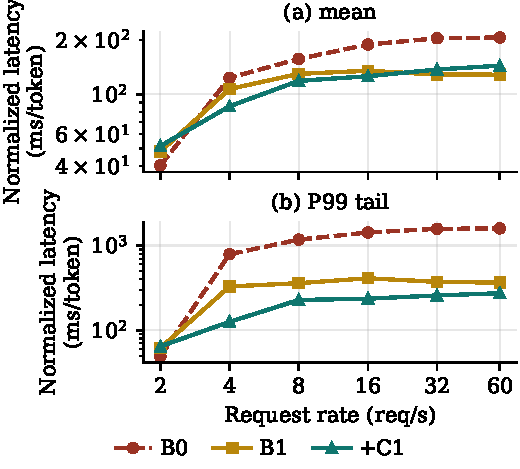
\includegraphics[width=\columnwidth]{fig7_nlatency_ladder.pdf}
  \caption{Reproduction of the LTR scheduling B1 on Engine A, trace, and metric. Normalized latency in milliseconds per generated token against arrival rate, for the unscheduled B0, the LTR, and the scheduler with cache compression C1. Panel (a) reports the mean and panel (b) the P99.}
  \label{fig:nlatency}
\end{figure}

When the request rate increases and the cache pool becomes full, the results diverge. The LTR scheduler (B1) reduces mean normalized latency compared with FCFS, and the P99 result improves more strongly because the scheduler reduces HOF blocking. This confirms that the earlier scheduling benefit is real. However, while it is not one fixed speedup number, the benefit depends on the offered load and the cache pressure.

The result shows LTR scheduler (B1) achieve 1.66 times on the mean and 3.6 times on the P99, and the reported 2.1 times sits between them~\cite{kumar2026}. The compression C1 shows a further improvement combined with LTR by paying a small per-token cost on the mean, but it cuts the tail by a further quarter, from 364 to 273 ms.

\subsection{Capacity Across Engine Versions}

Figure~\ref{fig:ladder} compares mean TTFT across three engine versions. The engines use different preemption strategies, but all three show the same general result: LTR scheduling improves TTFT, and cache compression improves it further.

At 64 requests per second, Engine A reduced mean TTFT from 4316 to 3160 ms with scheduling and to 925 ms with compression. Engine B reduced it from 5076 to 1423 ms with scheduling and to 939 ms with compression. Engine C reduced it from 12275 to 6488 ms with scheduling and to 2347 ms with compression.

The absolute numbers cannot be compared directly across engines, because the engines use different execution paths and cache formats. However, the same ordering appears in all three versions. This shows that the main benefit comes from increased cache capacity, not from one specific engine release or preemption implementation.

\subsection{Five-Configuration Comparison}

Figure~\ref{fig:fiveconfig} compares all five main configurations on Engine C at 64 requests per second. The scheduler reduces mean TTFT from 12275 to 6488 ms. Adding TQ4-bit cache compression reduces it further to 2347 ms. This is a large improvement, because more active requests fit into the same GPU memory.

However, compression increases mean TPOT from 68 to 215 ms, because the low-bit cache has to be unpacked and dequantized during decoding. Because of this cost, the compressed configuration has worse E2E latency than the scheduler-only configuration: 20708 ms compared with 15063 ms.

The BLASST sparsity method improves the compressed configuration. With compression and sparsity together, TTFT becomes 1747 ms, mean TPOT decreases from 215 to 167 ms, and mean E2E latency decreases from 20708 to 17308 ms. This result shows that compression helps the queueing and memory side, while sparsity helps the decode side.

\begin{figure*}[t]
  \centering
  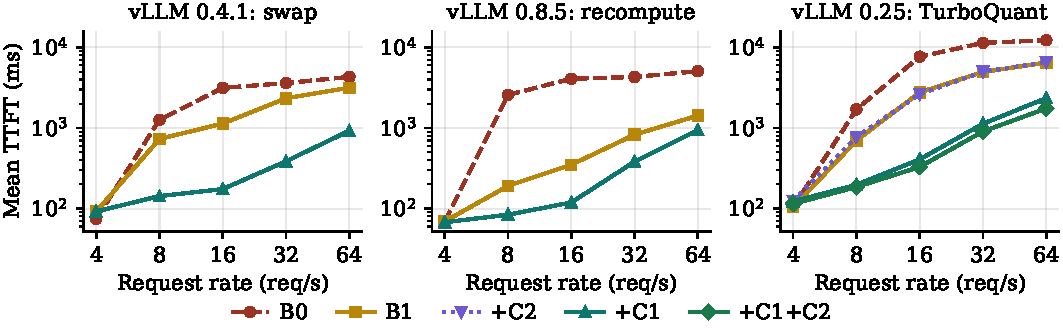
\includegraphics[width=\textwidth]{fig1_cross_engine_ladder.pdf}
  \caption{Mean time-to-first-token (TTFT), against arrival rate for the baseline (B0), the LTR scheduler (B1), and the scheduler with cache compression (B1+C1), on three engine versions with different preemption strategies (swap, recompute, and the current release). The third panel with Engine C adds the two BLASST sparsity arms with C1 (B1+C1+C2) and without C1 (B1+C2), which exist only on the release whose kernels we patched. The vertical axis is logarithmic, and absolute values are not comparable across panels; the ordering and shape are, and they are the same in all three.}
  \label{fig:ladder}
\end{figure*}

\begin{figure*}[t]
  \centering
  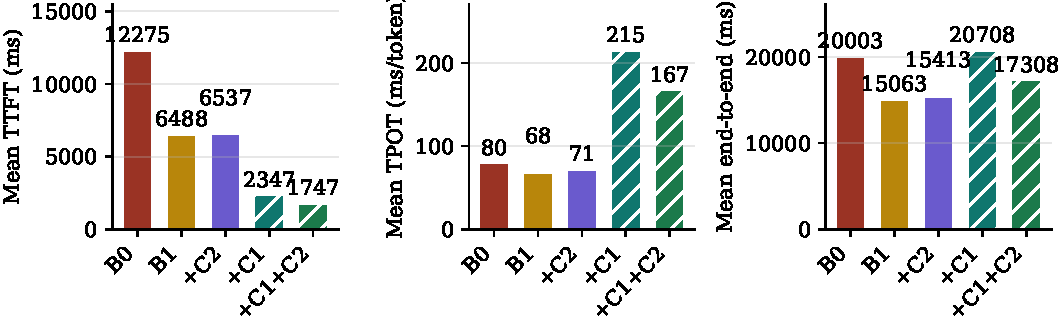
\includegraphics[width=\textwidth]{fig2_five_config_r64.pdf}
  \caption{The five configurations at 64 requests per second: mean time-to-first-token (TTFT), mean per-token latency (TPOT), and mean end-to-end (E2E) latency. Hatched bars use the TurboQuant 4-bit cache (C1), so the transition from solid to hatched is the compression step at equal device memory. Compression buys the TTFT and pays for it in the TPOT; BLASST sparsity returns the TPOT with combine with LTR (B1+C1+C2)}
  \label{fig:fiveconfig}
\end{figure*}

\subsection{Tail Latency Distribution}

Figure~\ref{fig:percentiles} shows the TTFT percentiles at 64 requests per second. The lower percentiles are similar across configurations, because a request that arrives when the system has free capacity can start quickly. The difference becomes large after the median P50.

\begin{figure}[H]
  \centering
  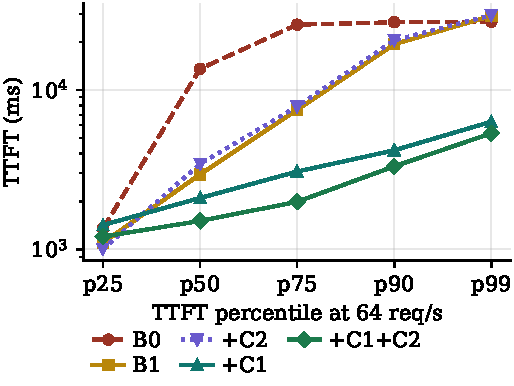
\includegraphics[width=\columnwidth]{fig3_ttft_percentiles.pdf}
  \caption{Time-to-first-token (TTFT) distribution of the five configurations at 64 requests per second, from the 25th to the 99th percentile, on a logarithmic axis. The curves separate by cache precision rather than by configuration: the three uncompressed arms (B0, B1, and B1+C2) converge above the median, while the two compressed arms (B1+C1 and B1+C1+C2) flatten the whole distribution}
  \label{fig:percentiles}
\end{figure}

The uncompressed configurations have P99 TTFT values between around 26800 and 29510 ms. Scheduling changes the order of the waiting requests, but it does not remove the memory bottleneck. The compressed configurations have much lower tail latency: the TQ 4-bit cache configuration reaches 6323 ms at P99, and the combined (B1+C1+C2) configuration reaches 5351 ms.

This result shows that compression does more than improve average performance. It flattens the latency distribution by reducing the number of requests that must wait for cache memory.

\subsection{Attention Sparsity Conditions}

Figure~\ref{fig:regimes} shows two conditions that affect the sparsity method. The first condition is the decode kernel design. On the bfloat16 unified grouped-query attention (GQA) kernel, adding sparsity increases mean TPOT by 4.9 \% and P99 TPOT by 15.0 \%. On the TurboQuant 4-bit per-head kernel, the same sparsity method reduces mean per-token latency by 22.1 \% and P99 latency by 46.8 \%.

The reason is kernel tiling. The GQA kernel shares one cache block across four query heads, so a block can only be skipped if the whole tile agrees that it is unimportant. This reduces realized sparsity from around 42 \% of identified blocks to around 18.5 \% of actually skipped blocks, and the overhead of the sparsity condition becomes larger than the work it saves.

The second condition is compute density. At a fixed arrival rate of six requests per second, sparsity improves TPOT by 20.4 \% at 512 context tokens and by 10.3 \% at 2048 tokens. At 4096 and 7168 tokens, the improvement disappears or becomes slightly negative. Long contexts reduce the active batch size, because each request consumes more cache memory, so the decode step becomes more bandwidth-bound and BLASST's skipping arithmetic does not help as much.

\begin{figure}[H]
  \centering
  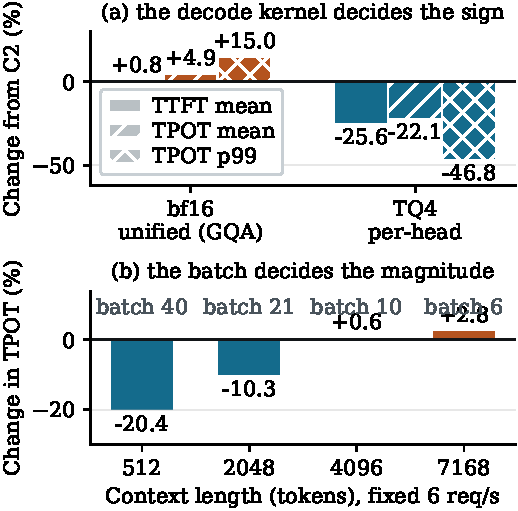
\includegraphics[width=\columnwidth]{fig4_c2_regimes.pdf}
  \caption{The two conditions on the sparsity lever, both as percentage change from adding it, so a bar below zero is an improvement and one above it a regression in each. Panel (a): one algorithm at one threshold helps on the per-head decode kernel and hurts on the kernel that shares a cache block across four query heads. Panel (b): at a fixed arrival rate the benefit fades as longer contexts shrink the batch and decode becomes bandwidth-bound, so it follows compute density rather than context length.}
  \label{fig:regimes}
\end{figure}

\begin{figure}[H]
  \centering
  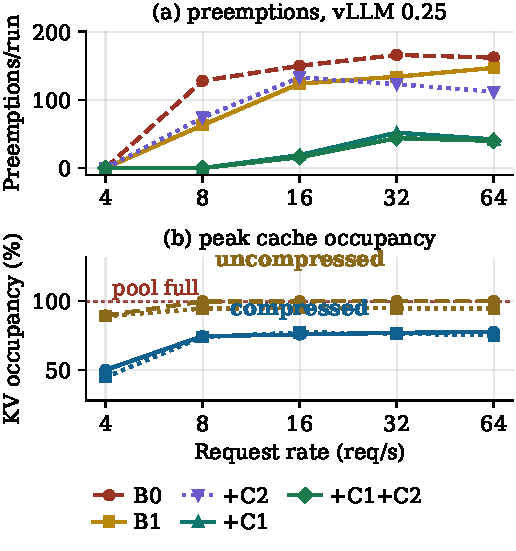
\includegraphics[width=\columnwidth]{fig6_preemptions.pdf}
  \caption{Panel (a) plots preemptions per run against request rate for all five configurations on Engine C, showing that compression, rather than ordering, removes most evictions. Panel (b) plots peak cache occupancy on both Engine A and B, which is instrumented identically on both; dotted curves are the swapping engine and solid or dashed are the recomputing. Both uncompressed arms reach the ceiling; compression holds both under 78 \% at every rate.}
  \label{fig:preempt}
\end{figure}

\subsection{Preemption and Cache Occupancy}

Figure~\ref{fig:preempt} measures the memory-pressure. At 64 requests per second, preemptions fall from 162 for FCFS (B0) to 147 for LTR scheduling (B1). With TQ4-bit cache compression (B1+C1), preemptions fall to 42, and with compression and sparsity (B1+C1+C2) together they fall to 40.

Scheduling reduces preemptions only slightly, because it improves request ordering but does not reduce the cache size. Compression removes most preemptions, because more requests fit into the KV cache pool. This supports the claim that cache capacity is the main reason for the large TTFT improvement.

The right side of Figure~\ref{fig:preempt} compares peak cache occupancy on the older engine versions. The uncompressed configurations reach 94.5 \% occupancy on the swapping engine and 100 \% occupancy on the recomputation engine, while the compressed configurations stay around 75.0 and 77.6 \%. This means that swapping and compression solve the same KV-cache problem in different ways: swapping handles cache overflow after it happens, while compression prevents the overflow from happening.

\subsection{Accuracy}

Table~\ref{tab:accuracy} shows GSM8K generation accuracy. The bfloat16 dense baseline achieves 0.80 accuracy. The bfloat16 sparsity configuration achieves 0.88, the four-bit cache configuration achieves 0.83, and the combined configuration achieves 0.85.

\begin{table}[H]
  \caption{Generation-based accuracy (GSM8K, $n=100$, greedy decoding).}
  \label{tab:accuracy}
  \centering
  \small
  \begin{tabular}{@{}lrr@{}}
    \toprule
    Configuration & GSM8K & $\Delta$ vs.\ bfloat16 \\
    \midrule
    bfloat16, dense (baseline) & 0.80 & --- \\
    bfloat16 + BLASST (C2)     & 0.88 & $+0.08$ \\
    TurboQuant-4bit (C1)       & 0.83 & $+0.03$ \\
    TQ4 + BLASST (C1+C2)       & 0.85 & $+0.05$ \\
    \bottomrule
  \end{tabular}
\end{table}

These results do not show evidence of accuracy degradation. However, the evaluation contains only 100 GSM8K problems, so a difference of several percentage points can represent only a few questions. We do not claim that quantization or sparsity improves accuracy. The correct conclusion is that tested configurations did not show measurable degradation in this sample

\clearpage
\section{Discussion}

The results show that KV-cache compression and attention sparsity work on different bottlenecks. Cache compression reduces memory usage, which lets more requests stay active and reduces TTFT, tail latency, and preemptions. However, compression adds per-token decode work, because the cache must be dequantized. Attention sparsity reduces some of this decode work by skipping blocks with non-effective softmax contribution

The combined configuration (B1+C1+C2) is better than compression alone (B1+C1) on the per-head decode kernel. TTFT improves from 2347 to 1747 ms, mean TPOT improves from 215 to 167 ms, P99 per-token latency improves from 1121 to 597 ms, and E2E latency improves from 20708 to 17308 ms. However, the combined configuration is not the fastest configuration for TPOT. The uncompressed scheduler-only configuration remains faster at 68 ms per token for TPOT, which is the cost of using low-bit cache storage.

Reproduction experiments are important. It confirms that LTR scheduling works on the original engine and workload. However, it does not mean that the same speedup scale will appear on every vLLM version. The old engine uses swapping, while the newer engine mainly uses recomputation. The cache compression result is more consistent, because it reduces the amount of cache memory needed before the preemption strategy matters. This is confirm since the Engine B upgrade over Engine A by vLLM team release versions when quantization becoming more popular.

One important finding is that sparsity is not only an algorithm problem. It is also a kernel implementation problem. The same threshold method helps the per-head kernel and hurts the GQA kernel. The GQA kernel shares cache blocks across multiple heads, so it cannot skip a block unless every grouped operation agrees, which reduces the real sparsity the kernel can use. Therefore, future sparsity papers should report both the identified sparsity and the realized kernel sparsity.

This work has some limitations. First, the experiments use one consumer RTX 3090 GPU. We cap the KV-cache pool to reproduce a memory-bound environment, but this is not the same as naturally reaching memory pressure on a datacenter GPU. Second, the evaluation uses one consistent seed, and absolute latency varies between runs, so the configuration ordering is more reliable than small numeric differences. Third, the two older engines use an 8-bit compression proxy instead of the native TurboQuant 4-bit configuration since vLLM do not have native TurboQaunt on older engines. Fourth, the sparsity implementation is only tested on the Engine A, because it was not ported to the older kernels. Finally, the sparsity threshold is fixed, while the original BLASST design scales the threshold with sequence length~\cite{blasst2025}.

\clearpage
\section{Conclusion}

This project built a KV-cache optimization layer under an LTR LLM scheduler and evaluated it as a complete serving system. TurboQuant 4-bit KV-cache quantization increased token capacity by 2.83 times at equal device memory, reduced mean TTFT at 64 requests per second from 12275 to 2347 ms, and reduced preemptions from 162 to 42 per run. BLASST Attention sparsity improved the compressed per-head decode kernel, reducing mean per-token latency by 22.1 \% and P99 per-token latency by 46.8 \%. However, the same method increased latency on a GQA kernel, because the kernel tile design limited the number of blocks that could be skipped. Overall, cache compression is most useful when serving is memory-bound, while attention sparsity is most useful when decode is compute-dense and the kernel can realize the identified sparsity.

\clearpage
\begin{figure}[H]
  \centering
  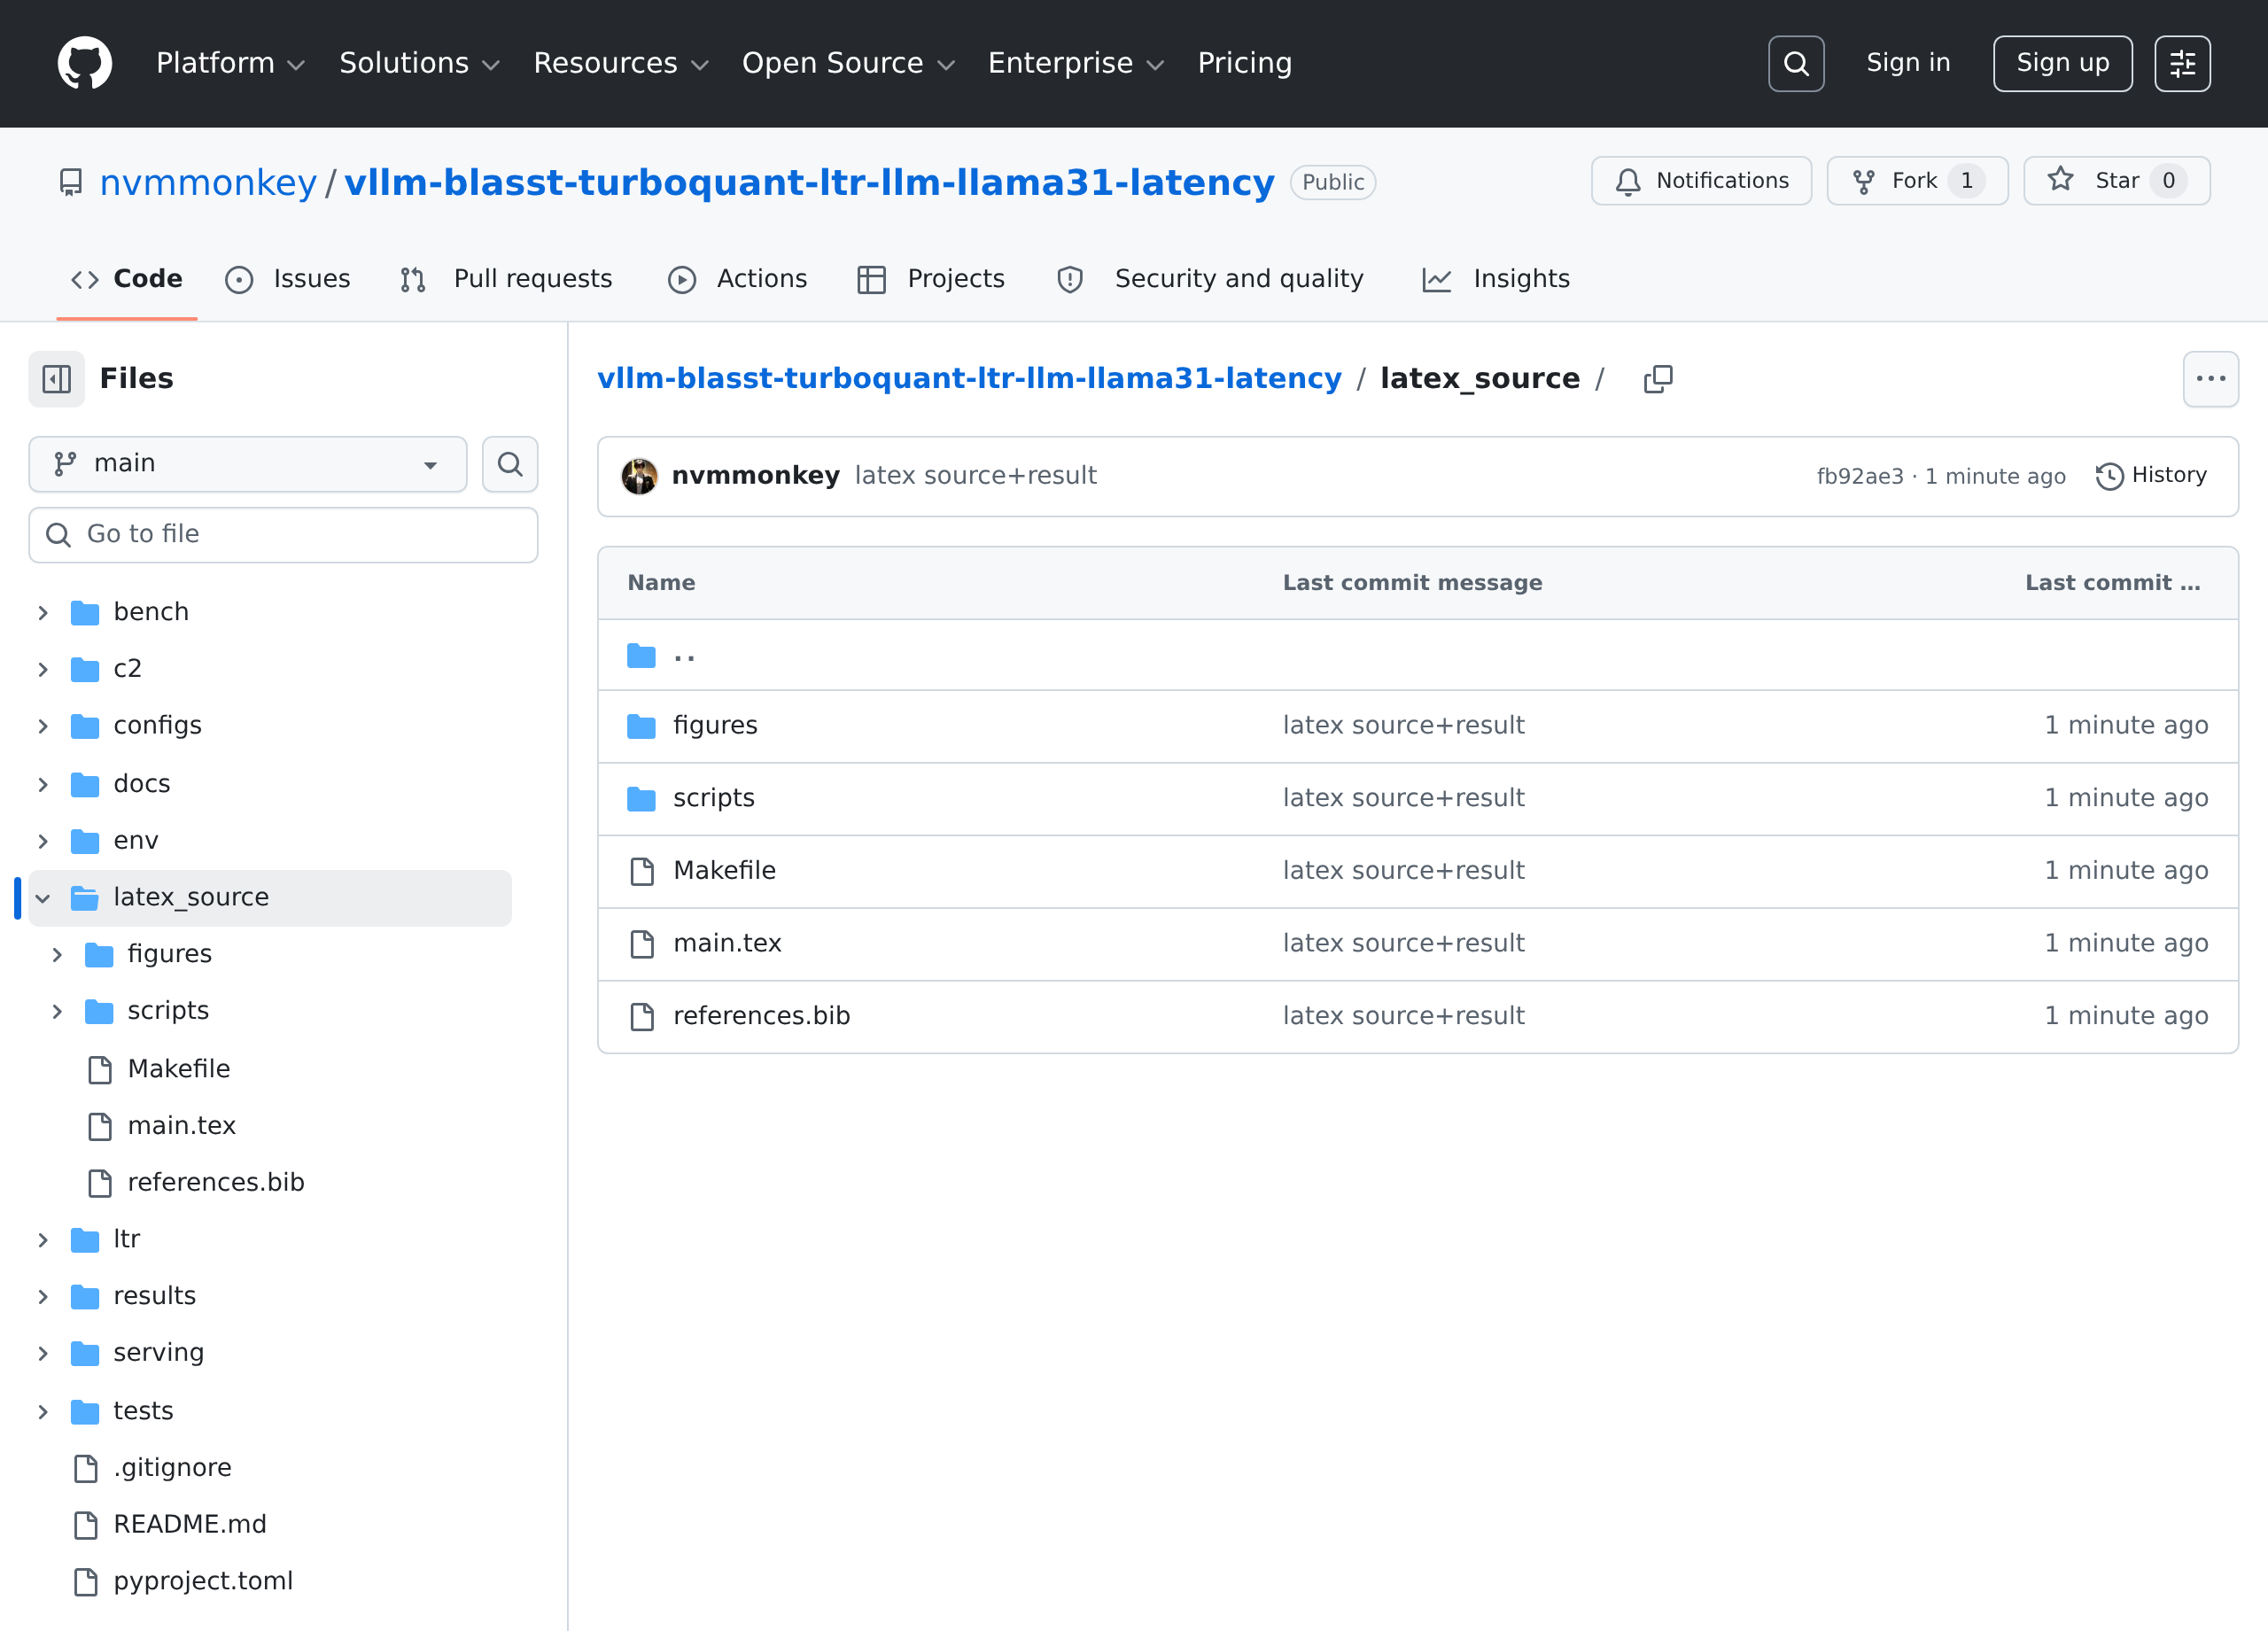
\includegraphics[width=\columnwidth]{latex_source_github.png}
  \caption{The \texttt{latex\_source} directory in the project repository.}
  \label{fig:appendix}
\end{figure}

\appendices
\section{}

Figure~\ref{fig:appendix} shows the latex\_source directory of this report in the project repository.

\clearpage
\bibliographystyle{IEEEtran}
\bibliography{references}

\end{document}
